\documentclass[conference]{IEEEtran}
\IEEEoverridecommandlockouts
% The preceding line is only needed to identify funding in the first footnote. If that is unneeded, please comment it out.
\usepackage{cite}
\usepackage{amsmath,amssymb,amsfonts}
\usepackage{algorithmic}
\usepackage{graphicx}
\usepackage{textcomp}
\usepackage{xcolor}
\usepackage{subcaption}
\usepackage{hyperref}
\usepackage[stable]{footmisc}
\usepackage{listings}


% -------------------------------------------------------------
% settings for code snippets

% \renewcommand{\lstlistingname}{Code Listing}  % Listing -> Code Listing
% \lstset{caption={Insert code directly in your document}}
% \lstset{label={lst:code_direct}}
% \lstset{basicstyle=\footnotesize}

% syntax highlighting
\definecolor{mygreen}{rgb}{0,0.6,0}
\definecolor{mygray}{rgb}{0.5,0.5,0.5}
\definecolor{mymauve}{rgb}{0.58,0,0.82}

\lstset{ %
    language=Python,
    frame=lines,
    backgroundcolor=\color{white},   % choose the background color
    basicstyle=\footnotesize,        % size of fonts used for the code
    breaklines=true,                 % automatic line breaking only at whitespace
    captionpos=b,                    % sets the caption-position to bottom
    numbers=left,                    % add line numbers
    commentstyle=\color{mygreen},    % comment style
    escapeinside={\%*}{*)},          % if you want to add LaTeX within your code
    keywordstyle=\color{blue},       % keyword style
    stringstyle=\color{mymauve},     % string literal style
    showstringspaces=false,
}


\def\BibTeX{{\rm B\kern-.05em{\sc i\kern-.025em b}\kern-.08em
    T\kern-.1667em\lower.7ex\hbox{E}\kern-.125emX}}
\begin{document}

\title{Chess Assignment\\
% {\footnotesize Introduction to Reinforcement Learning (Spring 2022). Source code available at
%  \href{https://github.com/TwoDigitsOneNumber/IntroRL_ChessAssignment}{https://github.com/TwoDigitsOneNumber/IntroRL_ChessAssignment}}
}

\author{
    \IEEEauthorblockN{van den Bergh Laurin}
    \IEEEauthorblockA{\textit{Institute of Informatics} \\
    \textit{University of Zurich}\\
    Zurich, Switzerland \\
    laurin.vandenbergh@uzh.ch | Matriculation number: 16-744-401}
}

\maketitle

\begin{abstract}
    % todo: remove red color
    \color{red}
    This document is a model and instructions for \LaTeX.
    This and the IEEEtran.cls file define the components of your paper [title, text, heads, etc.]. *CRITICAL: Do Not Use Symbols, Special Characters, Footnotes, 
    or Math in Paper Title or Abstract.
    1 sentence summary, 1 sentence method, and 1 sentence results, and 1 sentence conclusion.
\end{abstract}

\begin{IEEEkeywords}
    % todo: remove red color
    \color{red}
    reinforcement learning, chess
\end{IEEEkeywords}







\section{Introduction}\label{sec:introduction}

\subsection{- describe general setting}

In this assignment, we explore three different reinforcement learning algorithms to learn how to play a simplified version of chess. These three algorithms are SARSA, Q-Learning and DQN\footnote{SARSA serves as answer to task 3 and DQN serves as answer to task 5.}.


\subsection{- touch on methods}

Throughout the report we indicate in footnotes which task a particular section is referring to in terms of answering the task. We do this as the solutions to certain tasks are spread throughout multiple sections, e.g. task 3 is answered in Section~\ref{sec:methods} and Section~\ref{sec:results}. Even though this assignment was not solved in a group, we decided to also answer some of the ``group only'' and we stick to the numbering of the assignment in order to avoid confusion.

\subsection{- touch on results and conclusion}

seeds and nonseeded experiments foreshadow results from qlearning



\section{Methods}\label{sec:methods}


\subsection{Environment}

This version of chess takes place on a 4 by 4 board and can be thought of as a late game where the agent has a king and a queen, and the opponent has only a king. Since this game can only end in a win for the agent or in a draw, it is the agent's goal to learn how to win the game and avoid draws. For all experiments considered, the agent will be given a reward of 1 for winning, 0 for drawing, and 0 for all intermediate steps.

\textcolor{red}{For DQN no sequence is needed, because chess fulfills Markov property and gives rise to a Markov Decision Process (MDP). Also no preprocessing of sequence is needed anymore because state encoding is already given. \cite{atari2013} \cite{dqn2015}}

\textcolor{red}{Chess has/fulfills the Markov property, so applying reinforcement learning algorithms like Q-Learning and SARSA is theoretically justified.}





\textcolor{blue}{(1) Describe the algorithms Q-learning and SARSA. Explain the differences and the possible advantages/disadvantages between the two methods. No coding is needed to reply to this question.}


\subsection{SARSA and Q-Learning\footnote{Answer to task 1.}}


\subsubsection{Temporal-Difference Algorithms}
\textcolor{red}{maybe shorten}
SARSA and Q-Learning are two very related model-free types of temporal-difference (TD) algorithms for learning expected rewards, also known as Q-values, when rewards are not immediate and possibly sparse. The learning takes place via interaction with an environment through trial and error. These Q-values are in general represented by an action-value function Q and, for finitely many state-action pairs $(s,a)$, can be considered as a Q-table where each state-action pair, $(s,a)$, maps to a single Q-value, thus providing an estimate of the quality of any given state-action pair $(s,a)$. In this assignment however we use neural networks to approximate the action-value function, which outputs the Q-values for all possible actions for any given state. This helps to avoid computing large Q-tables. All algorithms explored in this assignment, including DQN, require the environment to fulfill the Markov property. \textcolor{red}{why? else what?}

\subsubsection{differences/what they have in common}
SARSA and Q-Learning address the temporal-credit-assignment problem \cite{sutton1984}, that is, trying to attribute future rewards to previous actions. These future rewards get discounted with the hyper-parameter $\gamma$ (see Section~\ref{sec:hyper-parameters}). Both algorithms repeatedly choose and take actions in the environment according to some policy $\pi$, e.g. an $\epsilon$-greedy policy.

However, this is where they differ.
SARSA is an on-policy algorithm, which means that consecutive actions are chosen according to the same policy $\pi$, even during the update step of the Q-values, which leads to the update rule: $$Q_\pi(s,a) \leftarrow Q_\pi(s,a) + \eta(r + \gamma Q_\pi(s_{t+1},a') - Q_\pi(s,a))$$ for some future action $a'$ chosen according to policy $\pi$.

Q-learning, on the other hand, is an off-policy algorithm, which means that it takes its actions $a$ according to its policy $\pi$, but during the update steps it assumes a greedy policy, i.e. optimal play, for future actions $a'$. 
Q-Learning has the update rule: $$Q_\pi(s,a) \leftarrow Q_\pi(s,a) + \eta(r + \gamma \max_{a'} Q_\pi(s_{t+1},a') - Q_\pi(s,a)).$$ 

\subsubsection{- advangages/disadvantages}
This leads to one of Q-Learning's major advantages: Because of Bellman's optimality equation, Q-Learning is guaranteed to learn the values for the optimal policy, i.e. $Q_*(s,a) = \max_\pi Q_\pi(s,a)$, and in a greedy stetting will take the optimal actions, at least if it was trained sufficiently. However, this can in certain cases mean that the online performance of Q-Learning will be worse than the one from SARSA, as Sutton et al. \cite{sutton2018} demonstrate with their ``gridworld'' example ``Cliff Walking''. Our chess game is a similar situation, because a win and a draw can be very close, thus during exploration Q-Learning can accidentally create a draw because it is going for the optimum when exploiting. Q-Learning is however relatively unstable and the parameters can even diverge when it is combined with non-linear function approximators \cite{dqn2015}, making the guarantee to learn the optimal policy irrelevant.

SARSA will learn to take a safer path, because it keeps its policy in mind when updating the Q-values, i.e. it keeps in mind that it will explore in future actions. This has the advantage that SARSA in general tends to explore more than Q-Learning.




\subsection{Experience Replay\footnote{Answer to ``group only'' task 2.}}

replay memory of fixed size, queue (get code in appendix)



\textcolor{blue}{(2) [Group Only] Describe the experience replay technique. Cite relevant papers.}

Experience replay is a technique proposed by Lin \cite{lin1992} to speed up the training process for reinforcement learning algorithms by reusing past experiences for future training. This is analogous to the human ability to remember past experiences and learn from them even after the fact. The past experiences are stored in a replay memory of fixed size at each time step $t$ as a tuple $e_t = (s_t, a_t, r_t, s_{t+1})$. 
% where $s$ denotes the state, $a$ denotes the action that was taken and $r$ denotes the received reward, each at some time step $t$. 
This essentially allows us to transform the learning process from online learning to mini-batch learning, where a batch of experiences $e_j$ is randomly sampled for each update step. Experience replay can only be used in combination with off-policy algorithms, because otherwise the current parameters determine the next sample and create unwanted feedback loops \cite{atari2013,dqn2015}.

Experience replay provides many benefits over online Q-Learning, especially when neural networks are used to approximate the action-value function. 
First, it enables the agent to learn from past experiences more then once, leading to increased data efficiency and faster convergence \cite{lin1992, atari2013}. Second, since for each update step past experiences are sampled randomly, the correlations between the individual actions are reduced, which then reduces the variance of the updates \cite{atari2013}. This leads to the experience samples $e_j$ being closer to i.i.d. and thus guaranteeing better convergence when using optimization algorithms such as stochastic gradient descent as most convergence proofs assume i.i.d. data.

\subsection{Deep Q-Networks (DQN)\footnote{Answer to task 5: Describing the used method.}}

A first version of the DQN algorithm was proposed by Mnih et al. \cite{atari2013} and combined experience replay with Q-learning, where a neural network was used as a non-linear function approximator for the action-value function. Mnih et al. \cite{dqn2015} later improved upon the method and presented the DQN algorithm, as it is known today, where they address the problem of the Q-values $Q(s,a)$ being correlated to the target values $y = r+\gamma \max_{a'} Q(s',a')$ because they are generated using the same neural network. In the DQN algorithm they separated the Q-network from the target network and only update the target network every $C$ steps, which helps to break this correlation and combat diverging network parameters. 


\subsection{Experiments}

In order to address all tasks, we divided the tasks into several independent experiments. First, we conducted seeded runs\footnote{Answers to task 3 and 5.} for all three algorithms using seed 21 for reproducibility, which was chosen a-priori. These seeded runs serve as examples to compare the algorithm's online performance qualitatively. The seeds are used such that the weights of all neural networks are instantiated identically for all algorithms and they subsequently serve as seeds for any random number used during training. This makes sure that all agents start with the same initial conditions and that the results are reproducible (see Section~\ref{sec:reproducibility}). All algorithms were run for 100000 episodes using identical model architecture and hyper-parameters (see Section~\ref{sec:implementation_hyper-parameters}).

Since the seeded runs are heavily influenced by the choice of the seed, we could end up with anything between a very lucky and well performing seed, or with a very unlucky one. Also the interpretation of the seeded runs is more difficult as we just have one run for each algorithm. Therefore, we decided to perform a simulation study and complete 30 non-seeded runs for each algorithm in order to get a better idea of how the algorithms perform on average. For computational reasons we limited these runs to 40000 episodes as we realized with test runs that by then most of the training progress has already taken place.

To analyze the impact of the hyper-parameters $\beta$ and $\gamma$\footnote{Answer to task 4.} we trained 49 agents with different combinations for $\beta$ and $\gamma$ but keeping all other hyper-parameters and model architecture identical. We chose SARSA for this experiment as we found it to have very low variance between its unseeded runs, which makes it an ideal candidate for comparing individual runs (see Figures~\ref{fig:30runs_reward} and \ref{fig:30runs_n_moves}). These runs are seeded identically to the seeded runs mentioned above.




\subsection{Implementation and Hyper-parameters}\label{sec:implementation_hyper-parameters}


\subsubsection{Implementation}

We implemented all algorithms from scratch according to Sutton et al. \cite{sutton2018} (SARSA and Q-Learning\footnote{SARSA as answer to task 3 and Q-Learning as additional algorithm.}) and Mnih et al. \cite{dqn2015} (DQN\footnote{Answer to task 5.}). For the implementation see file \verb"neural_net.py" on \href{https://github.com/TwoDigitsOneNumber/IntroRL_ChessAssignment}{GitHub} or Listing~\ref{code:neural_net}. All algorithms use a neural network with 58 input neurons, 200 hidden neurons and 32 output neurons, not including the biases for the input and hidden layer. The neural network automatically adds a constant input for the bias and the hidden layer. 
The implementation treats the biases like any other weights and thus they are part of any matrix multiplication. We used a ReLU activation function for the hidden layer and no activation on the output layer.
% A forward pass then looks like: $$ f(X) = g^{(2)}W^{(2)}g^{(1)}(W^{(1)}X), $$ where $X\in\mathbb{R}^{D+1\times N}$ represents the input.
The weights were initialized using Glorot initialization \cite{glorot2010}, such that the weights are sampled from a normal distribution with mean 0 and variance $\frac{2}{n_{\text{in}} + n_{\text{out}}}$, where $n_\text{in}$ and $n_\text{out}$ denote to the number of input and output neurons of the respective layer. This helped preventing exploding gradients for the most part.\textcolor{red}{check again with results}

\subsubsection{Hyper-Parameters}

For all experiments we used the default hyperparameters provided in the \verb"Assignment.ipynb" file unless otherwise noted.
For DQN we updated the weights of the target network after every $C=10$ steps, as most games take fewer steps than that. We used a replay memory of size 100000 and a batch size of 32.




\section{Results}\label{sec:results}

\subsection{Seeded Runs\footnote{Answer to task 3 (SARSA and Q-Learning as additional algorithm) and 5 (DQN).}}

\textcolor{blue}{(3) We provide you with a template code of the chess game. Fill the gaps in the
program file chess implementing either Q Learning or SARSA; detailed instructions
are available inside the file. We provide indicative parameter values. Produce two
plots that show the reward per game and the number of moves per game vs training
time. The plots will be noisy. Use an exponential moving average.}


The rewards and number of moves for the seeded runs are depicted in Figures~\ref{fig:rewards} and \ref{fig:n_moves} respectively. Since the curves are very noisy, we smoothed them using an exponential moving average (EMA) with a weight on the most recent observation of $\alpha = 0.001$.


\begin{figure}
    \centering
    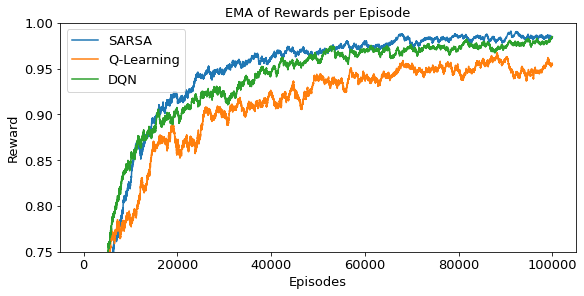
\includegraphics[width=.49\textwidth]{../figures/ema_rewards_per_episode_comparison.png}
    \caption{Exponential moving average of the rewards achieved during training. All three algorithms, Q-Learning, SARSA and DQN were initialized with identical weights and trained with identical network architecture and hyper-parameters.}
    \label{fig:rewards}
\end{figure}

\begin{figure}
    \centering
    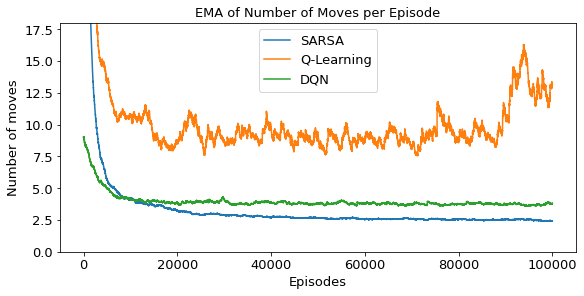
\includegraphics[width=.49\textwidth]{../figures/ema_number_of_moves_per_episode_comparison.png}
    \caption{\textcolor{red}{caption}}
    \label{fig:n_moves}
\end{figure}


As expected, the online performance of Q-Learning in terms of the rewards is generally lower than the rewards for SARSA but they converge slowly as $\epsilon$ decreases (Figure~\ref{fig:rewards}). Also in Figures~\ref{fig:rewards} and \ref{fig:n_moves} we can see that Q-Learning experiences instable learning behavior as both plots are a lot more noisy and at about 20000 and 90000 episodes the rewards decrease for some period. SARSA and DQN don't show this behavior.

Even though the number of steps is not punished, all agents still learn to reduce the number of steps over time, as they do not give rewards and their goal is to take actions that do. SARSA seems to do the best job at this, which perhaps is caused by its tendency to explore more and find better strategies. Q-Learning however seems to struggle to reduce the number of steps it takes.


\textcolor{blue}{(5) Implement another Deep RL algorithm (it could be SARSA if you chose before Q
Learning and vice versa). Compare the new results with your previous results.}

As suggested by Mnih et al. \cite{atari2013, dqn2015}, DQN\footnote{Answer to task 5 for comparing DQN to SARSA and Q-Learning.} was able to overcome the downsides of Q-Learning which lead to an online performance which is comparable to that of SARSA in terms of reward and number of moves it achieved, and also in terms of the stability during training. It did however not learn to reduce the amounts of steps as much as SARSA.


\subsection{Simulation Study (Non-seeded Runs)}

We can confirm that the qualitative results from the seeded runs reasonably well represent the average case. The only notable exception being Q-Learning, for which most runs performed equally well to the seeded run, but some runs experienced huge increases in the number of steps, which influenced the average run dramatically, leading to an average of about 23 moves per episode after 40000 episodes. For the learning curves see Figures~\ref{fig:30runs_reward} and \ref{fig:30runs_n_moves} in the Appendix. 

We observed that DQN and SARSA show very comparable learning curves with DQN showing slightly faster convergence in the first 5000 episodes. SARSA showed the lowest variance in all runs and seems to be a very stable algorithm. Q-Learning on the other hand showed clear signs of divergence as for some runs the rewards consistently dropped while the number of moves consistently increased. This shows that the measures taken by Mnih et al. \cite{dqn2015} to combat the disadvantages of Q-Learning worked and increased the stability as well as the convergence speed.

We can conclude that the seeded runs in our initial experiment truthfully represent the average run and therefore some level of inference is justified.

We also found out that, unsurprisingly, the effective training time is mainly dependent on the number of steps an algorithm takes per episode. This leads to Q-Learning having by far the longest training time, especially when the parameters diverge and the number of steps increase. DQN and SARSA have relatively short training times, with SARSA being the fastest.


\subsection{Hyper-parameters}\label{sec:hyper-parameters}



\textcolor{blue}{(4) Change the discount factor $\gamma$ and the speed $\beta$ of the decaying trend of $\epsilon$ (for a definition of $\beta$ please see code). Analyse the results.}


\subsubsection{gamma}
Figure~\ref{fig:hyper-parameters}(a) depicts the rewards and number of moves per episode as a function of $\beta$ and $\gamma$. We can see that the reward increases monotonically as $\gamma$ is increases, suggesting that a value of $\gamma\in[0.80, 1)$ should be chosen. This intuitively makes sense, as we have very sparse rewards and want the agent to ``backpropagate'' this reward through its sequence of actions. 

\subsubsection{beta}
We can not see a clear relationship between $\beta$ and the rewards, apart from $\beta=0$ being an inferior choice. In Figure~\ref{fig:hyper-parameters}(b) we can see that the that the number of steps taken by the agent decreases drastically when increasing $\gamma$ from very low levels, but again there is no clear pattern visible for $\beta$. In summary, for reasonalby chosen values of $\gamma$ the choice of $\beta$ seems to not have much of an influence for training periods up to 40000 episodes.

\begin{figure}
    \centering
    \begin{subfigure}[]{.5\textwidth}
        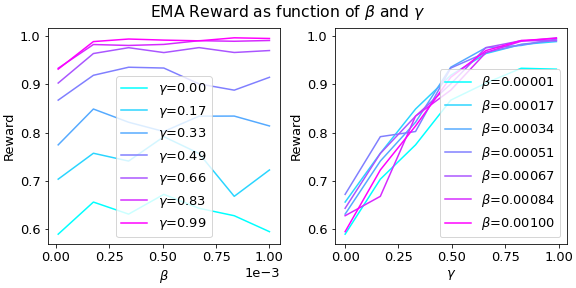
\includegraphics[width=\textwidth]{../figures/sarsa_Reward.png}
        \caption{}
    \end{subfigure}
    \begin{subfigure}[]{.5\textwidth}
        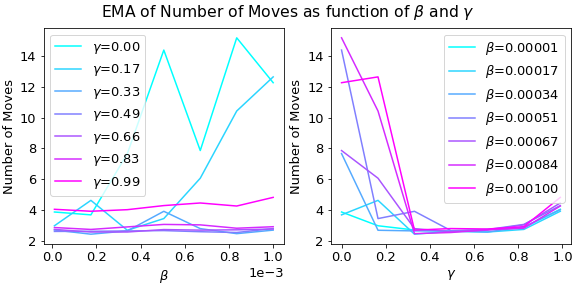
\includegraphics[width=\textwidth]{../figures/sarsa_Number of Moves.png}
    \end{subfigure}
    \caption{}
    \label{fig:hyper-parameters}
\end{figure}


\textcolor{blue}{(6) [Group Only] Change the state representation or the administration of reward. Interpret your results.}

\textcolor{blue}{(7) [Group Only] The values of the weights could explode during learning. This
issue is called exploding gradients. Explain one possible way to fix this issue and
implement it. For example, search and study RMSprop). Show in a plot how your
solution fixed this issue.}








\section{Conclusion}\label{sec:conclusion}

We are aware that the performance of the individual algorithms could be improved by tuning the hyper-parameters, however, this was not explicitly asked for and the focus on this assignment lies on the comparison of these algorithms.

summarize results, takeaway




\textcolor{red}{get correct bib format and complete entries}

\bibliographystyle{./IEEEtran}
\bibliography{./IEEEabrv,./Bibliography}

% \begin{thebibliography}{00}
%     \bibitem{atari2013} V. Mnih, K. Kavukcuoglu, D. Silver, D. Wierstra, A. Graves, I. Antonoglou, M. Riedmiller , ``Playing Atari with Deep Reinforcement Learning.'', CoRR, vol
%     % TODO: following entry is wrong
%     \bibitem{dqn2015} V. Mnih, K. Kavukcuoglu, D. Silver, D. Wierstra, A. Graves, I. Antonoglou, M. Riedmiller , ``Playing Atari with Deep Reinforcement Learning.'', CoRR, vol
%     \bibitem{sutton2018} R. S. Sutton and A. G. Barto, Reinforcement Learning: An Introduction., The MIT Press, 2018.

%     % todo: remove red color
%     \color{red}
%     \bibitem{b1} G. Eason, B. Noble, and I. N. Sneddon, ``On certain integrals of Lipschitz-Hankel type involving products of Bessel functions,'' Phil. Trans. Roy. Soc. London, vol. A247, pp. 529--551, April 1955.
% \end{thebibliography}

% todo: remove red color
\color{red}
\vspace{12pt}
IEEE conference templates contain guidance text for composing and formatting conference papers. Please ensure that all template text is removed from your conference paper prior to submission to the conference. Failure to remove the template text from your paper may result in your paper not being published.

\color{black}




\section{Appendix}
% todo: remove red color


\subsubsection{Reproducibility}\label{sec:reproducibility}


\textcolor{red}{put the appendix after the bibliography?}


\begin{figure}[htbp!]
    \centering
    \begin{subfigure}[]{.45\textwidth}
        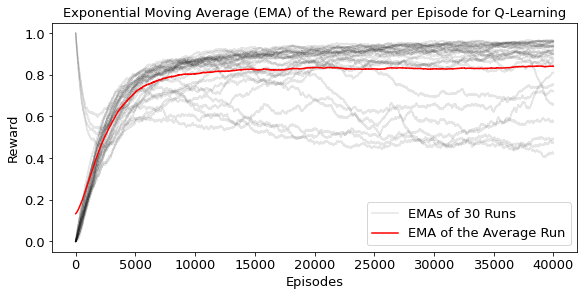
\includegraphics[width=\textwidth]{../figures/rewards_30_runs_qlearning.png}
        \caption{}
    \end{subfigure}
    \begin{subfigure}[]{.45\textwidth}
        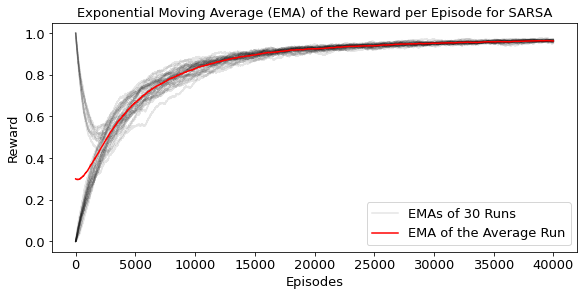
\includegraphics[width=\textwidth]{../figures/rewards_30_runs_sarsa.png}
        \caption{}
    \end{subfigure}
    \begin{subfigure}[]{.45\textwidth}
        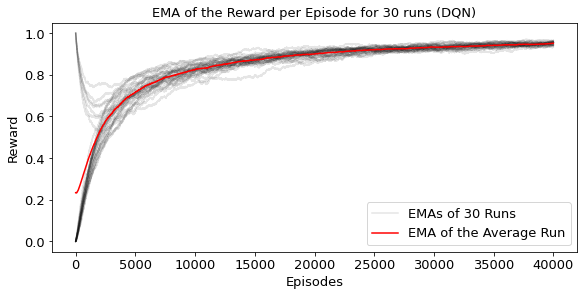
\includegraphics[width=\textwidth]{../figures/rewards_30_runs_dqn.png}
        \caption{}
    \end{subfigure}
    \caption{}
    \label{fig:30runs_reward}
\end{figure}
    

\begin{figure}[htbp!]
    \centering
    \begin{subfigure}[]{.45\textwidth}
        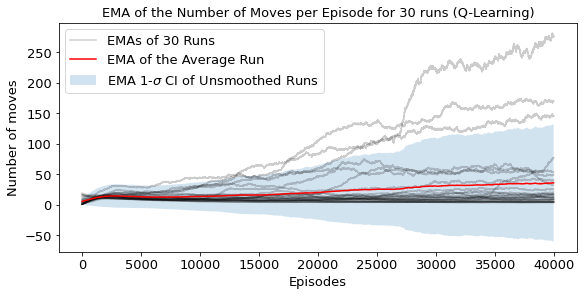
\includegraphics[width=\textwidth]{../figures/n_moves_30_runs_qlearning.png}
        \caption{}
    \end{subfigure}
    \begin{subfigure}[]{.45\textwidth}
        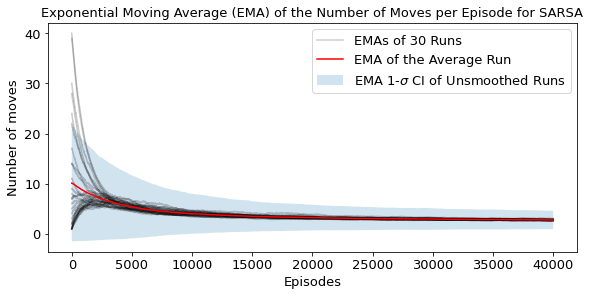
\includegraphics[width=\textwidth]{../figures/n_moves_30_runs_sarsa.png}
        \caption{}
    \end{subfigure}
    \begin{subfigure}[]{.45\textwidth}
        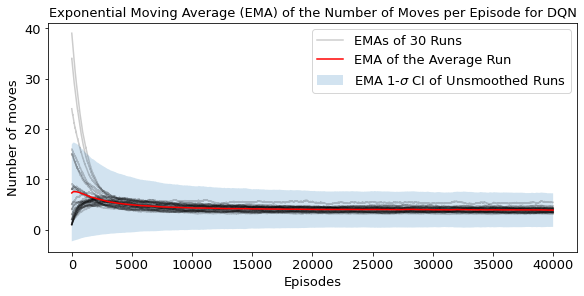
\includegraphics[width=\textwidth]{../figures/n_moves_30_runs_dqn.png}
        \caption{}
    \end{subfigure}
    \caption{}
    \label{fig:30runs_n_moves}
\end{figure}


\lstinputlisting[caption={\textcolor{red}{caption}}, label=code:neural_net]{../code/neural_net.py}


\end{document}